\documentclass[10pt]{article}
\usepackage[polish]{babel}
\usepackage[utf8]{inputenc}
\usepackage[T1]{fontenc}
\usepackage{amsmath}
\usepackage{amsfonts}
\usepackage{amssymb}
\usepackage[version=4]{mhchem}
\usepackage{stmaryrd}
\usepackage{graphicx}
\usepackage[export]{adjustbox}
\graphicspath{ {./images/} }
\usepackage{hyperref}
\hypersetup{colorlinks=true, linkcolor=blue, filecolor=magenta, urlcolor=cyan,}
\urlstyle{same}

\title{GIMNAZJUM }

\author{}
\date{}


\begin{document}
\maketitle
\begin{enumerate}
  \item Każda z liczb \(x_{1}, x_{2}, \ldots, x_{101}\) jest równa 1 lub -1 . Wyznacz najmniejszą możliwą wartość wyrażenia
\end{enumerate}

\[
x_{1} x_{2}+x_{2} x_{3}+x_{3} x_{4}+\cdots+x_{101} x_{1}
\]

\begin{enumerate}
  \setcounter{enumi}{1}
  \item Która z liczb jest większa \(3^{100}-2^{150}\) czy \(3^{50}-2^{75}\) ?
\end{enumerate}

Odpowiedź uzasadnij.\\
3. Czworokąt \(A B C D\) jest kwadratem. Wyznacz długość odcinka \(E C\), jeśli \(|A F|=4\) i \(|F B|=3 \mathrm{i}\) kąt \(A F E\) jest kątem prostym.\\
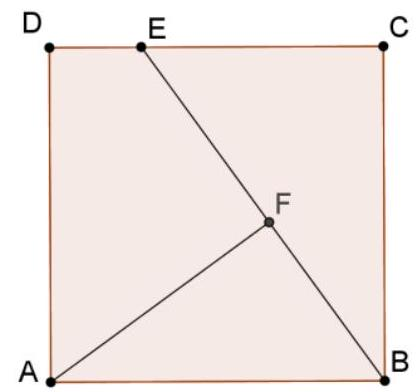
\includegraphics[max width=\textwidth, center]{2024_11_21_e8106a0b3aefeaed866dg-1}

\section*{LICEUM}
\begin{enumerate}
  \item Dana jest liczba rzeczywista \(a\), taka, że liczby \(a^{2}+a\) oraz \(a^{3}+a\) są wymierne. Udowodnij, że liczba \(a\) jest wymierna.
  \item Udowodnić, że jeśli \(a+b+c=0\) to \(a^{3}+b^{3}+c^{3}=3 a b c\).
  \item W trójkącie prostokątnym dane są długości jego przyprostokątnych. Na bokach zbudowano kwadraty, a następnie wyznaczono sześciokąt jak na rysunku. Oblicz pole tego sześciokąta.\\
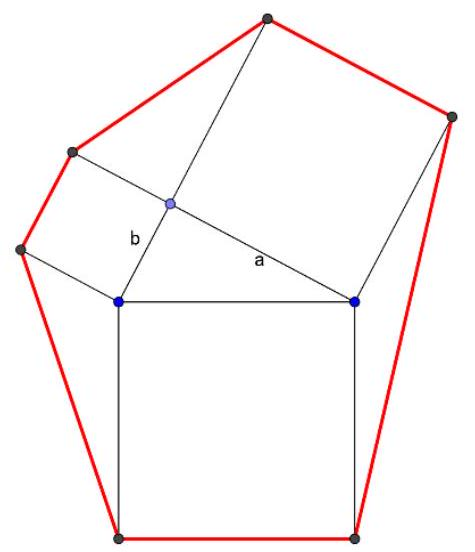
\includegraphics[max width=\textwidth, center]{2024_11_21_e8106a0b3aefeaed866dg-1(1)}
\end{enumerate}

Rozwiązania należy oddać do piątku 15 stycznia do godziny 12.00 koordynatorowi konkursu panu Jarosławowi Szczepaniakowi lub swojemu nauczycielowi matematyki lub przestać na adres \href{mailto:jareksz@interia.pl}{jareksz@interia.pl} do piątku 15 stycznia do pótnocy.


\end{document}